\section{Methodology}
Optimization of the nuclear fuel cycle is intended to develop 
a fuel cycle based on a specific objective or objectives. 
Optimization has previously been applied to the nuclear fuel 
cycle \cite{passerini_sensitivity_2012,andrianov_optimization_2019}
and other nuclear engineering \cite{chee_fluoride-salt-cooled_2022}.
This application of optimization uses \Cyclus \cite{huff_fundamental_2016}
to simulate the fuel cycle and Dakota \cite{adams_dakota_2019} to 
perform the optimization. In this chapter we demonstrate a methodology to 
apply this coupling to different optimization problems, and identify 
advantages and disadvantages of this methodology to optimize a nuclear 
fuel cycle. 

We developed three different optimization problems to apply to 
Scenarios 7 (no growth, once-through transition to the \gls{MMR}, Xe-100, 
and VOYGR) and 14 (no growth, limited recycling transition to the 
\gls{MMR}, Xe-100, and VOYGR): minimizing the \gls{SWU} capacity to 
produce \gls{HALEU}, minimizing the mass of \gls{SNF} for disposal, 
and minimizing both the \gls{HALEU} \gls{SWU} and the \gls{SNF} 
mass. To optimize these transitions, we consider six different 
variables: percent of \glspl{LWR} operating for 80 years (the \gls{LWR} 
lifetime), the build share 
of Xe-100s, the build share of \glspl{MMR}, the build share of VOYGRs, 
the discharge burnup of the Xe-100, and the discharge burnup of the 
\gls{MMR}. All of these variables were considered in the sensitivity 
analysis. The transition start time was also considered in the sensitivity 
analysis. However, that analysis showed that the transition start time has
very little effect on each of the metrics and delaying the transition 
can lead to unfulfilled energy demand. Therefore, this parameter is 
not considered in the optimization of each scenario. 

For this work, the percent of \glspl{LWR} operating for 80 years 
was constrained to between 0-50\% of the current \gls{LWR} fleet. 
The build share of each advanced reactor was allowed to range between 
0-100\%, but the three parameters had to sum to 100\%. The discharge 
burnups are restricted to the values considered in the \gls{OAT} 
sensitivity analysis.

We coupled \Cyclus \cite{huff_fundamental_2016} with Dakota 
\cite{adams_dakota_2021} to perform this optimization. For the 
single-objective problems, we used the ``soga'' solve method in 
Dakota, which is a single-objective genetic algorithm. For the 
multi-objective problems we used the ``moga'' solve method in 
Dakota, which is a multi-objective genetic algorithm. The Dakota 
User's Manual \cite{adams_dakota_2021} provides some guidance 
on selecting the most appropriate optimization method available 
in Dakota. According to this guide, these two methods are the most 
appropriate to use, because the problem has bound and linear constraints. 
Additionally, genetic algorithms
have previously been used to optimize fuel cycle transitions 
\cite{passerini_systematic_2014}. More specifically, the ``moga'' method 
in Dakota was found to always lead to a correct and accurate solution set 
when used with five different benchmark problems \cite{chiandussi_comparison_2012}.


Genetic algorithms are based on the survival of the fittest principle in 
evolutionary biology \cite{adams_dakota_2021}. The algorithm randomly 
selects an initial population of model parameters, with each set of model 
parameters forming a ``genetic string'' that is analogous to a DNA string 
that is unique for each member of a population \cite{adams_dakota_2021}.
Each member of a population is evaluated for its performance on a given 
problem, and the best performing sets of parameters are passed to the next 
generations, emulating the breeding of a population. In addition to 
passing along parameters sets to the next generation, crossovers and 
mutations occur. Crossovers are when one parameter value is exchanged 
between two members of the same population, similar to the combination of 
the genes from a parent to form a child \cite{kramer_genetic_2017}. In 
the crossover, the string of parameters are split at an arbitrary point, and 
switched to form two different offspring.
Mutations are when a parameter 
value of a population member is replaced with a random value within the 
parameter space. After mutation, the new population is evaluated for 
its performance in the defined problem. This process of 
crossover, mutation, and evaluation is performed for each population 
until a convergence criteria is met. Convergence criteria can be based on 
the convergence of a solution, the number of evaluations, or both. 

Genetic algorithms have a variety of hyperparameters, such as the the 
mutation rate and crossover rate, that can affect 
the results of the algorithm and the speed at which a solution is found. 
Specifically, the crossover and mutation rates of a genetic algorithm 
control how similar each population is to the one before it, and how much 
of new space is considered.If the mutation rate is too low, then the 
genetic algorithm can reach a local minimum instead of a global 
minimum. If the mutation rate is too high, then the algorithm behaves more 
like a random search and isn't able to fully use the information about the 
previous generation to find a minimum. If the crossover rate is too low, 
each generation is too similar to the one before it and the algorithm 
with converge without adequately exploring the parameter space. 
Therefore, before the genetic algorithms in Dakota can be used to 
optimize the fuel cycle transition, we must tune multiple hyperparameters
to determine the best combination for this work and the exact algorithm 
used by Dakota.

\subsection{Single-objective hyperparameter tuning}
We performed the tuning by performing a grid search across 
the possible values for some parameters, a method recommended 
by Deb \cite{deb_multi-objective_2001}, and used random 
search over other parameters. This method was demonstrated for reactor 
design optimization by Chee \cite{chee_fluoride-salt-cooled_2022}. 
Not all hyperparameters or all possible values of the hyperparameters 
were considered. We downselected from 
the possible hyperparameters and values defined in the Dakota Reference 
Manual based on hyperparameters defined in previous generic algorithms 
for nuclear energy applications
\cite{passerini_systematic_2014,chee_fluoride-salt-cooled_2022},
personal intuition, and limitations on time to perform 
the tuning.

The 
first grid search performed 40 iterations of different hyperparameter 
values across a coarse grid. The total number of samples was restricted to 
500 for each evaluation, which restricts the population size and the 
number of generations, as the product of these two must equal the 
total number of samples. Table \ref{tab:soga_tuning} describes 
the hyperparameters considered in the tuning and the range of possible 
values considered. Some of the variables, such as the mutation 
type, take discrete values while others, such as the crossover 
rate, can take continuous values. The crossover rate, mutation 
rate, and constraint penalty were treated as continuous for this 
tuning, and therefore were randomly sampled within the defined range. 
The population size can be a continuous variable, but was 
treated as discrete for this initial search to provide a well-defined 
number of generations. Hyperparameters not varied in the tuning, and 
help constant for all runs include the convergence type (kept at
``best fitness tracker'' ), the fitness type (kept at ``merit function''),
and the random seed (kept at the same value for all runs).

\begin{table}
    \centering 
    \caption{Hyperparameters and values considered in tuning. If a range 
    of values is provided, then the hyperparameter a random value in 
    that range was selected.}
    \label{tab:soga_tuning}
    \begin{tabular}{c c c}
        \hline
        Hyperparameter & Coarse Search & Fine Search \\
        \hline 
        Experiments [\#] & 1-40 & 41-60 \\
        Population size [\#] & 5, 10, 25, 50, 100 & 25, 50\\
        Constraint penalty & 0.5 $\leq$ x $\leq$ 2 & 1 $\leq$ x $\leq$ 2\\
        Crossover rate & 0.1 $\leq$ x $\leq$ 0.9 & 0.3 $\leq$ x $\leq$ 0.9\\
        Mutation type & replace uniform, offset normal & replace uniform, offset normal\\
        Mutation rate & 0.01 $\leq$ x $\leq$ 0.2 & 0.025 $\leq$ x $\leq$ 0.19\\
        \hline       
    \end{tabular}
\end{table}

All six of the input parameters considered were limited to integer
values by using the ``discrete design set'' variable definition for the 
Xe-100 and \gls{MMR} burnups and the ``discrete design range'' variable 
definition for the other four. This variable definition was selected to 
simplify file names and prevent rounding of values from Dakota.


Figure \ref{fig:soga_coarse_tuning} shows the results of the coarse tuning 
for the single objective problem. From these results, we observe that the 
\gls{HALEU} \gls{SWU} capacity tends to be lower with:
\begin{itemize}
    \item 
    \item 
\end{itemize}

\begin{figure}
    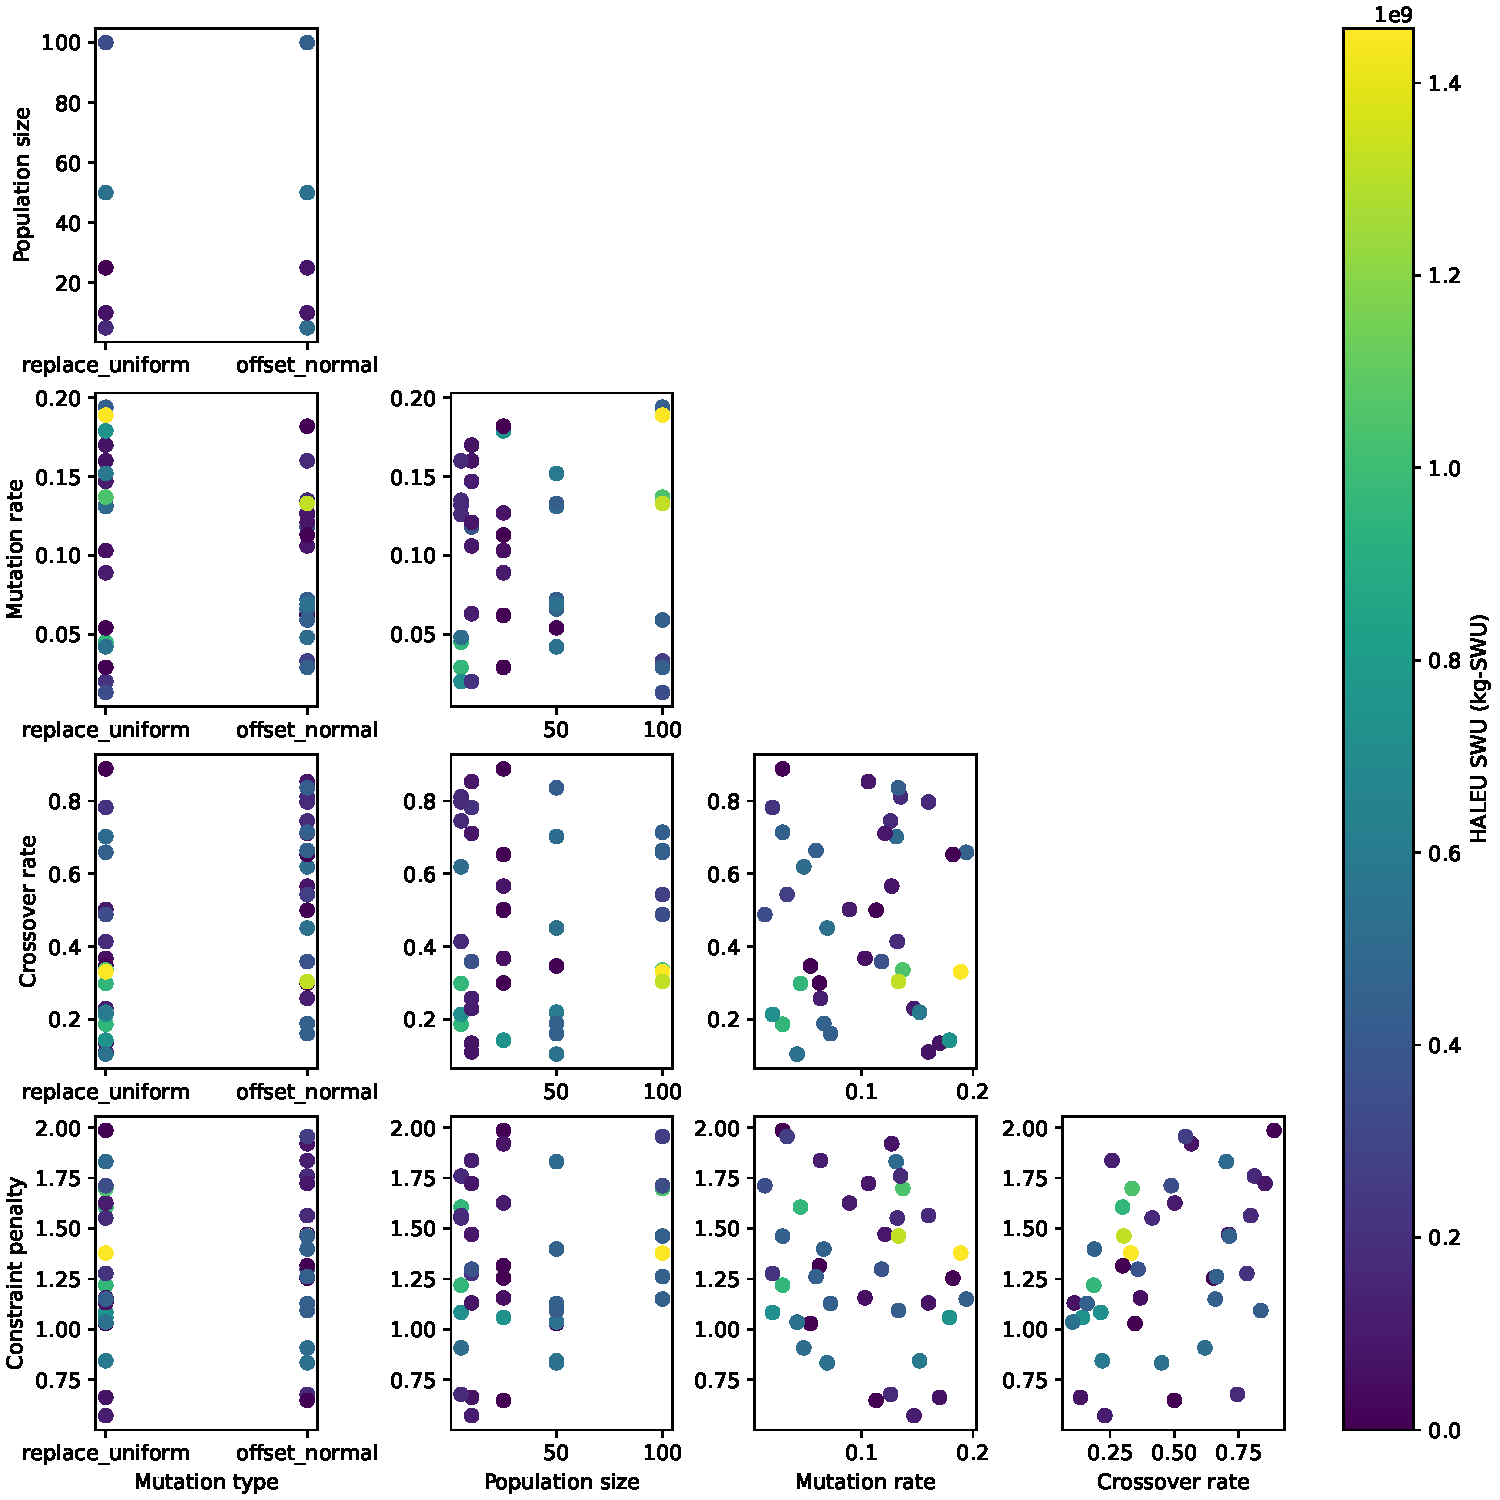
\includegraphics[scale=0.7]{soga_coarse_tunng.pdf}
    \caption{Results of coarse tuning for the single-objective 
    optimization.}
    \label{fig:soga_coarse_tuning}
\end{figure}



\subsubsection{Hyperparameter selection}
Table \ref{tab:soga_parameters} defines the hyperparameters used 
for all single-objective problems in this work.

\begin{table}
    \centering
    \caption{Hyperparameters selected for single-objective optimization.}
    \label{tab:soga_parameters}
    \begin{tabular}{c c}
        \hline
        Parameter & Value \\
        \hline
        Population & 25 \\
        Constraint penalty & 1.554\\
        Crossover rate & 0.753\\
        Mutation type & offset normal\\
        Mutation rate & 0.045\\
        \hline
    \end{tabular}
\end{table}

\subsection{Multi-objective hyperparamter tuning}
Hyperparameter tuning for a multi-objective problem is more complicated 
than tuning for a single-objective problem. In multi-objective 
problems, there is no single best solution but rather many solutions 
that form a Pareto front \cite{adams_dakota_2019}. The points on a 
Pareto front indicate that further improvement of one objective 
results in a worsening of another objective. Therefore, to tune the 
hyperparameters of a multi-objective problem, one tunes base on the 
hypervolume of the Pareto front \textbf{Find citation}. The 
hypervolume of a Pareto front is calculated by calculating the area 
between the Pareto front and a reference point. The reference point 
must be selected such that all values on the Pareto front are contained in 
the hypervolume. 

For multi-objective problems, we used the ``moga'' method in Dakota, which 
stands for Multi-objective Genetic Algorithm. Using this method, Dakota
outputs the Pareto front for the problem, which can then be used to 
tune the hyperparameters for this problem. 

We began by using the same problem and general sets of variable definitions 
as what was used for the ``soga'' runs: linear constraint, integers for 
all variables. We observed that by using a linear equality constraint
Dakota only found a single solution, as opposed to a Pareto front, because 
not all of the samples adhere to linear constraints. By using a linear 
inequality constraint, defining that the advanced reactor build share is 
at least 100\%, Dakota was able to provide values for a Pareto front. 
We then calculated the hyper volume 
for a given Pareto front. 

Hyperparameters selected for tuning in this work include the 
population size, the mutation rate, and the crossover rate. Each 
hyperparameter took specific values, instead of doing a random 
search of values, because of resource limitations. The population 
sizes considered include 10, 25, and 50, mutation rates considered 
include 0.08, 0.1, 0.15, \textbf{SOGA parameter}, and the crossover rates 
considered include 0.3, 0.8, and \textbf{SOGA parameter}. These values 
were selected based off of the hyper parameters used for the single-objective 
problem, the default value in Dakota, or intuition. The default values for 
the population size, mutation rate, and crossover rate are 50, 
0.08, and 0.8, respectively, in Dakota. Therefore, if the value of a 
hyperparameter is not specified, the Dakota default value is used.  
We ran each set of hyper 
parameters 20 times, and compared the statistics of the hypervolumes of 
the resulting Pareto fronts. From this data, we selected the 
hyperparameters to use for multi-objective optimization for this work. 





Not assigning any weights

\subsubsection{Hyperparameter selection}

\section{Once-through optimization}
\subsection{Minimize HALEU SWU}
By applying the hyperparameters to an optimization problem to minimize the 
\gls{HALEU} \gls{SWU} capacity needed by this transition scenario, Dakota
found a minimum with the values defined in Table \ref{tab:soga_ot_haleu}.

\begin{table}
    \centering 
    \caption{Values resulting in a minimum \gls{HALEU} \gls{SWU} capacity for 
              a once-through transition scenario.}
    \label{tab:soga_ot_haleu}
    \begin{tabular}{c c}
        \hline
        Variable & Value \\
        \hline
        LWR Lifetime & \\
        Xe-100 build share & \\
        MMR build share & \\
        VOYGR build share & \\
        Xe-100 burnup & \\
        MMR burnup & \\
        \hline
    \end{tabular}
\end{table}

\subsection{Minimize waste mass}
By applying the hyperparameters to an optimization problem to minimize the 
\gls{HALEU} \gls{SWU} capacity needed by this transition scenario, Dakota
found a minimum with the values defined in Table \ref{tab:soga_ot_waste}.
The minimum waste mass determined through the optimization is 22,703 MT. 

How well did this work? How important is it to tune the hyper parameters 
for each problem?

\begin{table}
    \centering 
    \caption{Values resulting in a minimum waste mass disposed of for 
              a once-through transition scenario.}
    \label{tab:soga_ot_waste}
    \begin{tabular}{c c}
        \hline
        Variable & Value \\
        \hline
        LWR Lifetime & 49.31\%\\
        Xe-100 build share & 85.93\%\\
        MMR build share & 6.53\%\\
        VOYGR build share & 9.31\%\\
        Xe-100 burnup & 185 MWd/kgU\\
        MMR burnup & 90 MWd/kgU\\
        \hline
    \end{tabular}
\end{table}

Each of the variables either match or trend towards expectations for this problem. 
Based on the transition analysis (Chapter \ref{ch:once_through_results}) and 
sensitivity analysis (Chapter \ref{ch:sa}), one would expect that to minimize 
the spent fuel mass the \gls{LWR} lifetime percent, Xe-100 build share, 
Xe-100 burnup, and \gls{MMR} burnup would all be maximized while the \gls{MMR} 
and VOYGR build shares are minimized with the deployment of \glspl{MMR} favored 
over VOYGR deployment. The Xe-100 and \gls{MMR} burnup values are at the maximum 
values considered for this work, which matches expectations. The \gls{LWR} lifetime 
extension percent is near the maximum considered for this work, which suggests that 
the waste mass from advanced reactors could be further decreased by using the 
maximum of this input parameter. 

The advanced reactor build shares trend towards expectations, but don't fully 
meet them. The deployment of Xe-100s over the other advanced reactors is consistent 
with the results in Table \ref{tab:nogrowth_waste}, which shows that only deploying 
Xe-100s results in less spent fuel mass than the other combinations of the reactors. 
Therefore, one would expect that the Xe-100 build share would be 100\%. Then combined 
with the other input parameters (the \gls{LWR} lifetime percent and Xe-100 burnup 
specifically) the optimized transition scenario would result in less spent fuel 
mass than the scenarios considered in Chapter \ref{tab:nogrowth_waste}.

\subsection{Minimize HALEU SWU and waste mass}

Results to include: graph of Pareto front

\section{Recycling optimization}
\subsection{Minimize HALEU SWU}

\subsection{Minimize waste mass}

\subsection{Minimize HALEU SWU and waste mass}
